\chapter{Einleitung}
\section{Aufgabenstellung}

Aufgabe dieser Studienarbeit ist es, mit Hilfe von Lego Mindstorms, einen Roboter aufzubauen. Dieser Roboter soll sich in einer ihm unbekannten Umgebung fortbewegen. Durch farbliche Objekte und Markierungen innerhalb dieser Umgebung soll er sich entsprechend derer Bedeutung verhalten. 

Des weiteren soll der Roboter soll der Roboter Hindernissen, wie Wänden, ausweichen können. 
\begin{figure}[htb]
\centering
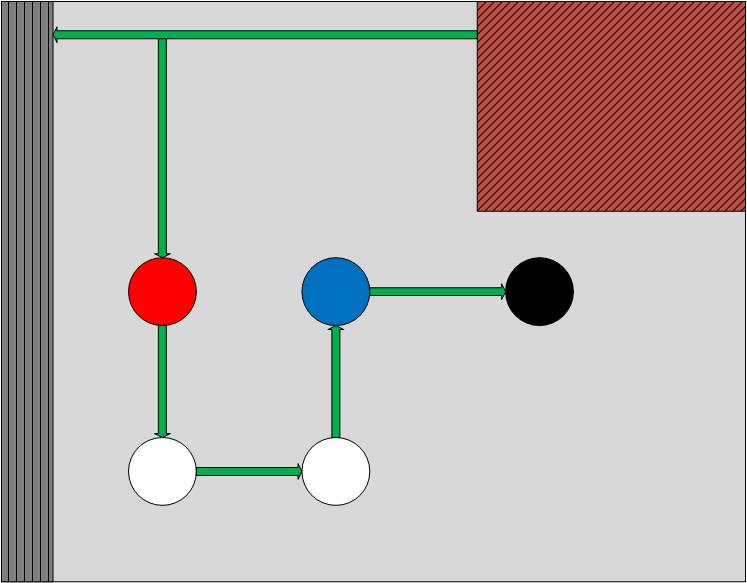
\includegraphics[width= 15cm]{parkur}
\caption{Übersicht des zu befahrenden Parkurs}
\label{fig:Fahrstrecke}
\end{figure}

Die Erkennung der farblichen Marikierungen soll mit Hilfe des mitgelieferten Farbsensors erfolgen. Die Wanderkennung soll mit Hilfe des Ultraschallsensors realisiert werden. 
Ein entsprechender Parkur, mit Markierungen und Hindernissen, ist der Abbildung \vref{fig:Fahrstrecke} zu entnehmen. In der Abbildung \vref{fig:legende} ist die entsprechende Legende, in der Symbole und Flächen näher erleutert.
\begin{figure}[htp]
\centering
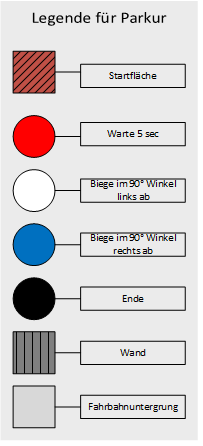
\includegraphics[width= 10cm]{legendeparkur.png}
\caption{Legende zu Bild \vref{fig:Fahrstrecke}}
\label{fig:legende}
\end{figure}

\section{Projektplanung}
\begin{table}[htp]
\centering
\begin{tabularx}{\textwidth}{|X|X|X|}
\cline{1-3}
  \textbf{ Dauer}&\textbf{Art der Tätigkeit}&\textbf{Meilenstein} \\\cline{1-3}
  1Woche& Einarbeitung & 1. Meilenstein\\\cline{1-3}
\end{tabularx}
\caption{Übersicht der Projektplanung}
\label{tab:projektplaung}
\end{table}
\textbf{Dies ist die Tabelle der Projektplanung}

\section{Verwendetet Software}
In diesem Projekt werden verschiedene Programmierumgebungen benutzt. Eine Programmierumgebung ist die Lego-eigene grafische Programmierumgebung. Diese Programmierumgebung gibt es in verschiedenen Ausführungen, genutzt wird die "LEGO MINDSTORMS Education EV3" Version. Diese IDE zeigt dem Nutzer unteranderem die aktuellen Werte der genutzten Sensoren an so wie deren Steckplatz am "Brick"\textbf{Glossareintrag}. Diese Programmierumgebung ist für den Einstieg und erste kleinere Programme geeignet, jedoch geht die Übersicht bei komplizierteren Programmen verloren. Aus diesem Grund wird in dieser Studienarbeit diese Umgebung dazu genutzt den Brick und die Funktionsweise der Sensoren näher kennen zu lernen. Dieses Wissen wird später dann auf die Java Programmierung transferiert.

Des weiteren wird die Java  IDE "Eclipse" mit der Erweiterung "Lejos" genutzt. Auf die Installation der Erweiterung wird im Anhang näher eingegangen. Diese Programmierumgebung \dots \\

Damit bei einem etwaigen Datenverlust der Verlust gering gehalten wird, wird die Versionsverwaltung GITHUB benutzt. Darin werden die Programme und auch dieses Dokument verwaltet. Bei einem Datenverlust kann somit auf eine vorhergehende  Version des Programms oder dieses Dokuments zurückgegriffen werden. Das verwendete Repository ist öffentlich und kann unter \url{https://github.com/saschlick/Studienarbeit/} eingesehen werden.\\Ebenso werden die gesamten Projektdaten in meiner DropBox gespeichert. Dies hat mehrere Vorteile. Zum einen kann ich an von jedem Computer mit Internetzugang darauf zugreifen und zum anderen ist es ebenfalls eine Absicherung gegen Datenverlust.     








